Image reconstruction is required to produce maps or images of activity distribution from the acquired tomographic measurements. Reconstruction algorithms used for this process can be categorised as either analytical reconstruction methods or statistical reconstruction methods.  
Analytical reconstruction methods seek to invert the transformation that links between image and data domain, using linear analytic approaches based on analytical formulations of the acquisition process. These methods treat the measured LOR data as line integrals over image space and necessitate corrections to be applied on projection data prior to reconstruction, in order to result to valid and quantitatively accurate images. The most commonly used analytical reconstruction method is the Filtered Back Projection which is described briefly in this chapter. 
Statistical reconstruction algorithms are derived from statistical formulations of the detection process and allow for the use of complex system models that account for the effects that result in degrading image quality and quantification.  These methods result in a non-linear formulation of the reconstruction problem which require iterative optimisation methods to reach a solution. The solution sought is a set of image parameters (that describe the activity distribution) which best describes the acquired projection data. 
In this thesis we made exclusive use of statistical reconstruction methods due to their ability to incorporate complex system models, including dynamic models which is imperative for the aims of this thesis.


\section{Projection and back-projection process}
Coincidence detection of annihilation photons in PET leads naturally to a line-integral model where the number of coincidence events is an \gls{lor} is approximately linearly proportional to the integral of tracer density along the volume joining the two detectors. 
In the simplified case of a 2D image space and a single ring 2D PET scanner, the projection process can be written as:
\begin{equation}
   \bm y = proj\{\bm{\lambda}\}  \\, 
  \label{eqn:Radon}
\end{equation}
where $\bm{\lambda}$ is the continuous distribution of radiotracer and $\bm{y}$ the continuous projection data (or else sinogram data). 
The projection operation is also known as the Radon transform~\cite{radon1917} and translates from the image to the projection data domain. 
The inverse operation is back-projection, which translates from data domain to image domain.

\subsection{Image representation}
In practice the spatio-temporal radiotracer distribution is described using a model of a finite number of parameters. The most common choice is the use of equally sized non-overlapping voxels that cover the useful \gls{fov}. Their use extends also to the temporal domain where each temporal bin is described independent of each other. 
If for a moment we only consider the spatial domain, we can model the spatial radiotracer distribution $\bm{\lambda}$ using voxels with the  $rect$ function as
\begin{equation}
   g(\bm{r};\bm\lambda) = \sum_{j=1}^{n_{j}} \lambda_j {rect}(\bm{r}-\bm{r}_j)  \\, 
\end{equation}
for ${n_{j}}$ voxels, with $r_j$ coordinates and intensity $\lambda_j$.
For the case where the model is linear as in this case, the set of functions describing the distribution are referred to as 'basis functions'. We will be using the $\bm\lambda$ notation to refer to the ${n_{j}}$ vector of  $\lambda_j$ voxel weights that describe the spatial activity distribution. 
\begin{equation}
   \bm\lambda = \Big\{ \lambda_j,j=1..n_j \Big\} \\.
\end{equation}
Regarding the temporal aspect of the activity distribution, traditionally the data are binned temporally (in frames), with each considered as an individual acquisition. This leads to a similar modeling for the image data, where the $rect$ function is used for each frame, set from the frame start and frame end time points. In this project we explore and use additional types of modeling the dynamic aspect of activity distributions, which are described in more detail in the following sections. For the image data representation it is common to separate the temporal aspect as a separate index. The activity distribution can be written as
\begin{equation}
   \bm{\lambda} = \Big\{ {\bm{\lambda}_m,m=1,...,n_m} \Big\} \\,
\end{equation}
where
\begin{equation}
   \bm{\lambda_t} = \Big\{ {\lambda_{tj},j=1,...,n_t} \Big\} \\.
\end{equation}
Equivalently the projection space is also effectively modeled according to the discretization imposed by the \glspl{lor} as $y_i,i=1..n_i$, where $i$ is the projection bin index and $n_m$ the total number of \glspl{lor}. For multiple time frames we define $y_{mi}$ as the number of events for bin $i$ at frame $m$ for a number of $n_m$ frames. The dynamic data can then be written as
\begin{equation}
   \bm{y} = \Big\{ {\bm{y}_m,m=1,...,n_m} \Big\} \\,
\end{equation}
where
\begin{equation}
   \bm{y_m} = \Big\{ {y_{mi},i=1,...,n_i} \Big\} \\.
\end{equation}


\subsection{Projection}
Projection of image to data space can be treated by summing contributions of voxels across each projection ~\gls{lor}. Different projection strategies exist that model the contribution of voxels differently depending on their placement in the \gls{lor}. As this is a computationally heavy process in practice, different methods have been proposed that balance between accuracy and consistency and computing requirements. A short follows list with basic description of the methods that are implemented in CASToR.

\begin{itemize}
\item  \textbf{Siddon projector}~\cite{Siddon1985}: Weights the contribution of an LOR to each by the length of the line that intersects the voxel.
\item  \textbf{Distance driven}~\cite{DeMan2004}: An optimised method for calculating weights by mapping pixel boundaries and detector boundaries for each projection to a common axis .
\item  \textbf{Incremental Siddon}~\cite{Jacobs2015}:
\item  \textbf{Joseph}~\cite{Joseph1982}: Estimates contribution of voxels to LOR based on linear interpolation and their distance from the LOR. 
\item  \textbf{Multi-Siddon}~\cite{Moehrs2008}: Uses multiple lines from the faces of the detectors in each LOR to approximate the volume intersected between the two detectors and the voxel.
\end{itemize}

\begin{figure} [h!]
\centering
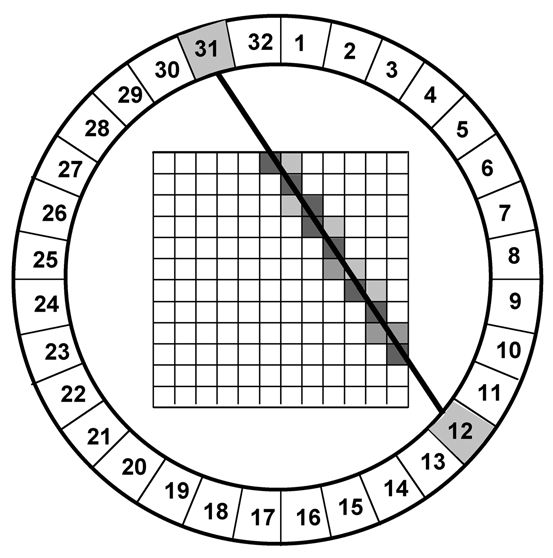
\includegraphics[scale=0.35,angle=0]{2_Theory_Methods/figures/Radon_Discrete.png}
\caption{Back-projection of a single LOR through image space, with contribution weighted according to the length of the line that intersects the voxel.} 
\label{fig_3:back_projection.}
\end{figure} 

The inverse process of back-projection assigns the contribution from each bin across the \gls{lor}, using the same strategies described above. 
Analytical reconstruction methods estimate an image though the process of back-projecting all the data in image space where the contributions from all \glspl{lor} are superimposed. In practice a filtered version of the projections is back-projected to account for the non-uniform number of contributions from LORs in differnt regions of the image space, which gives the processes the name of filtered back projection. The method can be extended to 3D via use of the 3D X-ray transform and approximations of missing data projections~\cite{Kinahan1989}. 

But while analytical reconstruction are linear processes that result to estimates at relatively little computing time, accuracy is limited by the assumptions of the line integral model, positron range effects, variations in response across an LOR etc. In addition these methods do not account for the statistical properties of the data. They assume noise-free data and equal weighting between LORs, which for noisy data results to image artefacts that necessitate post reconstruction smoothing and processing.

\section{Formulation of the system model}
One main advantage of iterative reconstruction methods is the ability to make use of complex models that map the radiotracer distribution from image space to data space, which can include physical processes such as positron range, scatter and random contributions, attenuation effects, normalisation factors etc.
The projection process described above can be modelled using a matrix $\bm{X}$ of $n_i$x$n_j$ dimensions. This is the projection or system matrix and each ${X}_{ij}$ element is the average probability of detecting an emission from voxels site $j$ at the data bin $i$. With that the projection of an image $\bm{\lambda}$ at bin $i$ can be written as a sum over the contribution of all voxels from the image
\begin{equation}
   \hat{y_i} = \sum_{j=1}^{n_j} X_{ij} \lambda_j  ,
\end{equation}
where $\hat{y_i}$ is the modelled data or expectation of the data.  A more realistic system model can be expressed as 
\begin{equation}
   \hat{y_i} = \sum_{j=1}^{n_j} A_{i}N_{i}X_{ij} \lambda_j + B_{i} \\,
\end{equation}
where vectors $A$ and $N$ account for attenuation and efficiency factors at bin $i$ , and $B$ for scatter and randoms which are modelled as additive terms. In addition \gls{psf} modeling can be included to model voxel value at voxel j using a \gls{psf} model. 
For shortness all the effects can be written as a matrix $P$ and the system model can be re-written as
\begin{equation}
   \hat{y_i} = \sum_{j=1}^{n_j} P_{ij} \lambda_j + B_{i} \\.
   \label{eqn:system_model}
\end{equation}

\section{Formulation of the objective function}
The second most important advantage of iterative reconstruction methods is the inherent accounting for the statistical variations in the detection process This is achieved by the use of a probabilistic model in the derivation of the objective function, which is used in the optimisation process of the iterative reconstruction algorithm.
The total number of detection from annihilation photons in each projection bin can be modelled as a random sample from a Poisson distribution. According to the Poisson probability model, the conditional probability or likelihood function for $\hat{y_i}$ given the measured data ${y_i}$ will be
\begin{equation}
p({y_i}|{\hat{y_i}}) = L({\hat{y_i}}|{y_i}) = e^{-\hat{y_i}} \frac{\hat{y_i}^{y_i}}{{y_i}!}  \\  .
\end{equation}
With the assumption that measurements of counts in each bin are independent random processes, the likelihood of the data over all bins will be
\begin{equation}
p(\bm{y}|\bm{\hat{y}}) = L(\bm{\hat{y}}|\bm{y}) = \prod_i e^{-\hat{y_i}} \frac{\hat{y_i}^{y_i}}{{y_i}!} 
\label{eqn:probability}
\end{equation}
By substituting equation \ref{eqn:system_model} in equation~\ref{eqn:probability} , we can write an expression of likelihood of the image $\bm{\lambda}$ given the measured data $\bm{y}$.
\begin{equation}
    L(\bm{\lambda}|\bm{y})  = \prod_i e^{-(\sum_{j=1}^{n_j} P_{ij} \lambda_j + B_{i} )} \frac{(\sum_{j=1}^{n_j} P_{ij} \lambda_j + B_{i} )^{y_i}}{{y_i}!}
\end{equation}It is more convenient to take the expression of the log likelihood in the following derivation. Since the log function is monotonic, the likelihood $L$ and its log $logL$ can be used to arrive to the same solutions when used as cost functions.The log likelihood expression is
\begin{equation}
    lnL(\bm{\lambda}|\bm{y})  = \sum_{i=1}^{n_i}\left[  -\sum_{j=1}^{n_j} (P_{ij} \lambda_j + B_i) + y_i ln(\sum_{j=1}^{n_j} P_{ij} \lambda_j + B_i) - ln({y_i}!) \right] \\.
\label{eqn:log_likelihood}
\end{equation}
This expression is the famous  "Poisson log-likelihood"  which will be used to arrive to the maximum likelihood estimate image $\bm\lambda$, which will be noted as $\bm{\lambda}^{ML}$, that maximises the likelihood of the modelled data given the measured data  $\bm{y}$


\section{Expectation Maximisation}
We can seek to solve equation~\ref{eqn:log_likelihood)} to find directly the maximum likelihood image $\bm{\lambda}^{ML}$ by taking its first partial derivative to $\lambda_j$ to be equal to zero. 
\begin{equation}
\frac{\partial lnL(\bm{\lambda}|\bm{y})}{\partial \lambda_j} = \sum_{i=1}^{n_i}\left[  -\sum_{j=1}^{n_j} P_{ij} + 
y_i \frac{\sum_{j=1}^{n_j} P_{ij} }{\sum_{j=1}^{n_j} (P_{ij} \lambda_j + B_i)}
\right]  = 0 \\. 
\end{equation}
By ignoring the constant term, this expression simplifies to 
\begin{equation}
\sum_{i=1}^{n_i}\left[  -\sum_{j=1}^{n_j} P_{ij} + 
y_i \frac{\sum_{j=1}^{n_j} P_{ij} }{\sum_{j=1}^{n_j} (P_{ij} \lambda_j + B_i)} \right]  = 0 \\,
\end{equation}
which has no closed form solution. The arrival to this expression shows that the statistical modelled reconstruction requires iterative methods to find the $\bm{\lambda}^{ML}$ solution. The most common algorithm used for this problem is the Expectation Maximisation algorithm that was first applied on the statistical PET reconstruction by two key works by Shepp and Vardi~\cite{Vardi1985} and Lange and Carson~\cite{Lange1984}. In these works the solution is derived though the introduction of the "complete data" concept~\cite{Dempster1977}. The complete data is an unknown dataset of $z_{ij}$ values which describes the exact number of emissions from voxel $j$ that contribute to the measurement at projection bin $i$. This is an unknown dataset, but the \textit{expectation} of the complete dataset can be expressed by taking measured data $\bm{y}$ and an image estimate (a guess) noted as $\bm{\lambda}^{(k)}$, as a ratio of fractions
\begin{equation}
\frac{z_{ij}}{y_i} = 
\frac{P_{ij} \lambda_j^{(k)}}{\sum_{d=1}^{n_j} (P_{id}\lambda_d^{(k)} + B_i)} \\,
\end{equation}
which is set by the ratio between complete data and measured (incomplete) data for a projection bin $i$, arising from voxel $j$, to be equal to the fraction of their modelled means which is calculated from the current estimate of the data image  $\bm{\lambda}^k$. From this expression the conditional expectation of the complete complete data is given by
\begin{equation}
\hat{z}_{ij}(\bm{\lambda}^{(k)},y_i) = 
\frac{P_{ij} \lambda_j^{(k)}}{\sum_{d=1}^{n_j} (P_{id}\lambda_d^{(k)} + B_i)}y_i\\.
\end{equation}
for which the log-likelihood expression becomes
\begin{equation}
lnL(\bm{\lambda}|\bm{\hat{z}})  =
\sum_{i=1}^{n_i} \sum_{b=1}^{n_j} \left[ -(P_{ib} \lambda_b) + \hat{z}_{ib} ln( P_{ib} \lambda_b ) - ln(\hat{z}_{ij}!) \right] \\,
\label{eqn:log_likelihood_z}
\end{equation}
for which the maximum can be found by partial differentiation to $\lambda_j$, resulting in the solution:
\begin{equation}
\lambda_j^{(EM)} = \frac{\sum_{i=1}^{n_i} \hat{z}_{ij} }{\sum_{i=1}^{n_i} P_{ij} } \\.
\label{eqn:EMupdate}
\end{equation}
This solution provides a new image estimate which maximises the expectation of the complete data, and is referred as the EM image. 
Together with the expression for the conditional expectation of the complete data, the two step process of Expectation Maximisation and  Maximum likelihood estimation can be written in a single update equation. Given data $\bm{y}$ and an image estimate $\bm{\lambda}^{(k)}$ , the updated image estimate $\bm{\lambda}^{(k+1)}$ is given from:
\begin{equation}
\lambda_j^{(k+1)} = \frac{\lambda_j^{(k)}}{\sum_{i=1}^{n_i} P_{ij}} 
\sum_{i=1}^{n_i} P_{ij} 
\frac{y_i}{\sum_{d=1}^{n_j} P_{id}\lambda_d^{(k)} + B_i } \\.
\label{eqn:MLEM}
\end{equation} 
This equation forms a single update of the MLEM algorithm, which when evaluated over all voxels $j$ provides an updated image $\bm{\lambda}^{(k+1)}$. 
The use of the conditional expectation of the data is in fact an example of the general concept of optimisation transfer, where the construction of surrogate functions is made to be used with simpler optimisation process, that leads to optimisation of the main function as well.

\section{Fully 4D reconstruction}
\label{section:Fully_4D_reconstruction}
Soon after the proposition of the EM algorithm for iterative PET reconstruction by Shepp and Vardi~\cite{Vardi1985} and Lange and Carson~\cite{Lange1984}, the former group proposed an extension of the EM algorithm to update parameters of a dynamic model and a version of the update algorithm that iterates through the whole of dynamic PET data in each iteration~\cite{Carson1985}. Dynamic PET data are traditionally divided among many time bins (frames) resulting in limited counts in each bin. Reconstruction of each bin and post-reconstruction kinetic modeling results in noisy and potentially biased parameter estimates. Furthermore the noise in each frame image estimate is spatially correlated and is hard to be accounted for in the post-reconstruction modelling. The use of an EM approach that updates over parameters using all the dynamic PET raw data offers the advantages of accurate noise modeling of the raw data and accurate system modeling directly in the process of parameter estimation. Unfortunately one major disadvantage of this approach was very slow convergence properties making it difficult for use in practice~\cite{Carson1985}. \\
More than 10 years later the approach was revisited by Mathews \textit{et al}\cite{Matthews1995} where it was combined with linear models. As it will be shown bellow the EM algorithm can be easily extended to parametric space with use of linear models. There the benefits in reducing parametric image noise were seen, at the cost of slow convergence. For use with linear models, attempts to accelerate convergence were made by use of OSEM~\cite{Tsoumpas2008} and computing acceleration and compression techniques~\cite{Hong2008}. In the case of fully 4D reconstruction with OSEM it was shown that the algorithms exhibits the “traditional” OSEM problem of limit-cycles, for which an decreasing subsets scheme was used to eliminate this effect~\cite{Angelis2011}. \\
It was not until the work of two groups in 2010, Wang \textit{et al}~\cite{Wang2010} and Matthews \textit{et al}~\cite{Matthews2010}, that allowed for practical and more widespread use of 4D reconstruction. Their methods, based on principles of optimisation transfer principles by Lange~\cite{Lange2000}, decouple 4D reconstruction to an EM update over all data and to an ML problem in image space. The first step iterates though the data and updates the activity estimate images, while the second simply updates the model parameters over the  updated activity images. With the second step being much faster, multiple dynamic model updates can be conducted for each update over data and result in acceleration of overall convergence. Results were demonstrated by Wang \textit{et al}~\cite{Wang2010} for EM and PCG based optimisations using linear models~\cite{Wang2010}. While that work was limited to linear dynamic models, the work by Matthews \textit{et al} generalised on the optimisation of the image space ML problem by the use of an equivalence to a weighted least-square minimisation problem~\cite{Matthews2010}. This formulation allowed for use of existing LS optimisation algorithms, which are commonly used for post-reconstruction model fitting, to be used in 4D reconstruction with both linear and non-linear models. The disadvantage of this approach is that the resulting ML formulation is not concave and thus does not guarantee monotonic convergence to a global maximum. Nevertheless convergence behaviour has been observed in practice with different weighting schemes~\cite{Gravel2015,Wang2013}. \\
The used of non-linear models with 4D reconstruction has shown clear benefits in precision and accuracy~\cite{Angelis2014,Kotasidis2012,Gravel2015}, but are more sensitivity to initialisation and reconstruction parameters and could lead to unpredictable behaviour.



\section{Optimization transfer}
%We then seek to find the estimate $\bm{\lambda}$ which maximises the log-likelihood equation~\ref{eqn:log_likelihood},
\begin{equation}
\argmax{\bm{\lambda}}lnL(\bm{\lambda}|\bm{y}) \\, 
\end{equation}
by taking advantage of optimisation transfer transfer principles (and avoiding the use of the missing data concept). We seek to find a surrogate $Q(\bm{\lambda}|\bm{\lambda}^{(k)})$ based on a estimate/guess of the activity distribution $\bm{\lambda}^{(k)}$ , for which : 
\begin{equation}
L(\bm{\lambda}|\bm{y}) \geq Q(\bm{\lambda}|\bm{\lambda}^{(k)}) 
\end{equation}
Then the optimisation can be split in the two steps: 
\begin{itemize}
\item Expectation: Find function $Q(\bm{\lambda}|\bm{\lambda}^{(k)})$ 
\item Maximisation: Update estimate $\bm{\lambda}^{(k+1)}$ from $\argmax{\bm{\lambda}} Q(\bm{\lambda}|\bm{\lambda}^{(k)})$ 
\end{itemize}
For a convex function $f$:
\begin{equation}
f(\sum_i \alpha_i x_i ) \leq \sum_i \alpha_i f(x_i )\quad  \text{for}  \quad \sum_i \alpha_i = 1,\quad  \alpha_i \geq 0
\end{equation}
and thus for two vectors $\bm{c}$ and $\bm{w}$ with positive components $c_i$ and $w_i$, 
\begin{equation}
f(\bm{c}^t \bm{v}) \leq \sum_i \frac{c_iw_i}{\bm{c}^t\bm{w}}f(\frac{\bm{c}^t\bm{w}}{w_i}v_i)
\label{eqn:optimisation_transfer}
\end{equation}
if we set $f$ to be the $-ln$ function, $\bm{c}^t$ as $\sum_j P_{ij} $ and $\bm{v}$ as $\bm{\lambda}$ in equation \ref{eqn:simpleloglikelihood} we have: 
\begin{equation}
    lnL(\bm{\lambda}|\bm{y})  \geq \sum_i \left[  -\sum_j (P_{ij} \lambda_j) + y_i  \sum_j \frac{P_{ij} \lambda^{(k)}_j}{\sum_k P_{ik} \bm{\lambda}^{(k)}} ln(\frac{\sum_k P_{ik} \bm{\lambda}^{(k)}}{\lambda^{(k)}_j} \lambda_j ) - ln({y_i}!) \right]
\end{equation}
\begin{equation}
\geq \sum_i \left[  -\sum_j (P_{ij} \lambda_j) + y_i  \sum_j \frac{P_{ij}\lambda^{(k)}_j}{\sum_k P_{ik} \bm{\lambda^{(k)}}} ln(\frac{\sum_k P_{ik}  \bm{\lambda}^{(k)}}{\lambda^{(k)}_j} \lambda_j )  \right]
\end{equation}
\begin{equation}
= \sum_i \left[  -\sum_j (P_{ij} \lambda_j) + y_i  \sum_j \frac{P_{ij}\lambda^{(k)}_j}{\sum_k P_{ik} \bm{\lambda}^{(k)}} (ln(\sum_k P_{ik} \bm{\lambda}^{(k)}) - ln(\lambda^{(k)}_j) + ln( \lambda_j ) )  \right]
\end{equation}
\begin{equation}
= \sum_j \left[  -\sum_i (P_{ij} \lambda_j) + \sum_i y_i \frac{P_{ij}\lambda^{(k)}_j}{\sum_k P_{ik} \bm{\lambda}^{(k)}} ln( \lambda_j )  \right]  + \underbrace {\sum_j  \sum_i y_i \frac{P_{ij}\lambda^{(k)}_j}{\sum_k P_{ik} \bm{\lambda}^{(k)}} (ln(\sum_k P_{ik} \bm{\lambda}^{(k)})- ln(\lambda^{(k)}_j))}_{const}
\end{equation} 
\begin{equation}
\geq \sum_j \left[  -\sum_i (P_{ij} \lambda_j) + \sum_i y_i \frac{P_{ij}\lambda^{(k)}_j}{\sum_k P_{ik} \bm{\lambda}^{(k)}} ln( \lambda_j )  \right]  
\end{equation} 
\begin{equation}
=  \sum_j Q(\bm{\lambda}|\bm{\lambda}^{(k)})
\end{equation} 

Which satisfies: 
\begin{equation}
\frac{\partial }{\partial \lambda_j} Q(\bm{\lambda}|\bm{\lambda}^{(k)})|_{\lambda=\lambda^{(k)}} = \frac{\partial }{\partial \lambda_j} lnL(\bm{\lambda}|\bm{y})|_{\lambda=\lambda^{(k)}}
\end{equation} 

The surrogate function can now can be maximised :
\begin{equation}
\bm{\lambda}^{(k+1)} = \argmax{\bm{\lambda}}Q(\bm{\lambda}|\bm{\lambda}^{(k)}) 
\end{equation}
\begin{equation}
\frac{\partial }{\partial \lambda_j} Q(\bm{\lambda}|\bm{\lambda}^{(k)}) = \sum_j \left[  -\sum_i P_{ij}  + \sum_i y_i \frac{P_{ij} \lambda^{(k)}}{\sum_k P_{ik} \bm{\lambda}^{(k)}} \frac{1}{\lambda_j}  \right]  
\end{equation}

, set to zero to find the value of $\lambda$ that maximises the function, $\bm{\lambda} = \bm{\lambda}^{(k+1)}$
\begin{equation}
0 =  -\sum_i P_{ij}  + \sum_i y_i \frac{P_{ij} \lambda^{(k)}}{\sum_k P_{ik} \bm{\lambda}^{(k)}} \frac{1}{\bm\lambda^{(k+1)}} 
\end{equation}
\begin{equation}
\sum_i P_{ij} =  \sum_i y_i \frac{P_{ij} \lambda^{(k)} }{\sum_k P_{ik} \bm{\lambda}^{(k)}} \frac{1}{\bm\lambda^{(k+1)}} 
\end{equation}
\begin{equation}
\bm\lambda^{(k+1)} = \frac{\bm\lambda^{(k)}}{\sum_i P_{ij}} \sum_i P_{ij} \frac{y_i}{\sum_k P_{ik} \bm{\lambda}^{(k)}}
\end{equation}


\section{Dynamic reconstruction - NestedEM}
As described in \textit{Image representation}, the common model used for describing and discretizing the radiotracer distribution is the voxel, where for dynamic data they are extended to individual sets of voxels for each temporal bin. 
As described in section \textit{Kinetics}, dynamic data are used to seek parameters of a kinetic model that aims in explaining the behaviour of the pharmacokinetics. Conventionally the data of each frame are reconstructed individually in individual 3D reconstructions and the result images are used for post-reconstruction modelling. When the parameters sought are calculated at the voxel level, the result is a set of parameters for each voxel of the 3D reconstruction voxels, which are referred to as parametric maps. If we an example dynamic model that describes the dynamic evolution of the radiotracer distribution with parameters $\theta_{pj}$ of $p=1..n_p$ parameters for each voxel $j$, we can write the radiotracer activity distribution as 
\begin{equation}
   \lambda_{tj} = f_{tj}(\bm\theta_{j}) \\,
\end{equation}
where $f()$ is the function of the dynamic model that estimates radiotracer activity values over $n_t$ time frames given a set of $n_{p}$ parameters $\bm\theta_{j} =  \Big\{\theta_{1j},...,\theta_{n_{p}j} \Big\}$.
Considering that the dynamic model is the same for all voxels in the image space, we can write for short 
\begin{equation}
\bm\lambda = f(\bm\theta) \\, 
\end{equation}
with the complete spatio-temporal distribution being 
\begin{equation}
   \bm{\lambda} = \Big\{ {{\lambda}_{tj},t=1,...,n_t ; j=1,...,n_j} \Big\} \\. 
\end{equation}
The dynamic model $f()$ can be either linear or non-linear to the set of parameters. 
When the spatio-temporal data $\bm{\lambda}$ are reconstructed form individual 3D frame reconstructions they commonly result to high noise in the activity distribution images due to the limited counts in each time frame. When  the dynamic model parameters are sought or parametric images, the dynamic or kinetic model is fitted post-reconstruction. Especially in the case of parametric images the noise of the individual 3D frame data results to noisy and potentially biased parametric images. This two step process not only results in noise parametric images but also does not account for the noise in the PET data in the post-reconstruction fitting process. 
Instead of this two-step process, it is possible to derive reconstruction algorithms that include dynamic models and can be applied on the whole of the dynamic PET data. These reconstruction algorithms, which are referred to as 4D reconstruction algorithms due to their application in 4 dimensions, seek to reduce the problem of limited counts that would else be used in individual frame bins by making use of the whole of the dynamic PET data. The dynamic models used are chosen to provide meaningful constrains and when the model of interest that would otherwise be used post-reconstruction is included, the 4D reconstruction algorithms can directly provide the parameters and parametric images of interest. 
Typically (although its not always the case) the number of parameters of dynamic models is smaller than the number of time frames in a study and so the use of 4D reconstruction effectively reduces the number of parameters to estimate, that along with the constraints imposed by the dynamic model result in an important reduction of noise and potentially improved bias. Furthermore direct use of dynamic models in reconstructions allows for the use of the noise-model that describes the PET data detection to be accounted for in the estimation of the final dynamic model parameters. 

\subsection{4D reconstruction optimisation}
Using the generic dynamic model $f()$ the conditional expectation of the complete complete data is given by 
\begin{equation}
\hat{z}_{tij}(\bm{\theta}^{(k)},y_{ti}) = 
\frac{P_{ij} f_j(\bm\theta^{(k)})}
{\sum_{d=1}^{n_j} (P_{id} f_d(\bm\theta^{(k)} + B_{ti})}y_{ti}\\,
\end{equation}
and the log-likelihood by
\begin{equation}
lnL(\bm{\theta}|\bm{\hat{z}})  =
\sum_{t=1}^{n_t} \sum_{i=1}^{n_i} \sum_{b=1}^{n_j} 
\left[ -P_{ib} f_b(\bm\theta^{(k)}) + B_{ti} + 
\hat{z}_{tib} ln( P_{ib}  f_b(\bm\theta^{(k)}) + B_{ti} ) -
ln(\hat{z}_{tij}!) \right] \\.
\end{equation}
For the maximisation of this function the constant terms can be ignored and so 
\begin{equation}
\bm{\theta}^{(k+1)} = \argmax{\bm{\theta}}(lnL(\bm{\theta}|\bm{\hat{z}})) = 
\sum_{t=1}^{n_t} \sum_{i=1}^{n_i} \sum_{b=1}^{n_j} 
\left[ -P_{ib} f_b(\bm\theta^{(k)}) + 
\hat{z}_{tib} ln( f_b(\bm\theta^{(k)})) 
\right] \\, 
\end{equation}
\begin{equation}
\bm{\theta}^{(k+1)} = \argmax{\bm{\theta}}(lnL(\bm{\theta}|\bm{\hat{z}})) = 
\sum_{t=1}^{n_t} \sum_{b=1}^{n_j} \left[ \sum_{i=1}^{n_i}  P_{ib} \right]
\left[ -f_b(\bm\theta^{(k)}) + 
ln( f_b(\bm\theta^{(k)})) 
\frac{\sum_{i=1}^{n_i} \hat{z}_{tib} }
{ \sum_{i=1}^{n_i}  P_{ib} }
\right] \\ .
\end{equation}
Where similarly to \ref{eqn:EMupdate}, the last part of the expression is equivalent to an EM update over data of frame $t$ and voxel $b$ as 
\begin{equation}
\frac{\sum_{i=1}^{n_i} \hat{z}_{tib} }
{\sum_{i=1}^{n_i}  P_{ib}}  =
\frac{f_j(\bm\theta^{(k)})}{\sum_{i=1}^{n_i}  P_{ib}}
\sum_{i=1}^{n_i} 
\frac{y_{ti}}
{\sum_{d=1}^{n_j} P_{id} f_d(\bm\theta^{(k)}) + B_{ti}}\\.
\end{equation}
This image can be referred to as the EM update image 
\begin{equation}
f_{tj}^{(EM)}(\bm{\theta}^{(k)}) = 
\frac{f_j(\bm\theta^{(k)})}{\sum_{i=1}^{n_i}  P_{ib}}
\sum_{i=1}^{n_i} 
\frac{y_{ti}}
{\sum_{d=1}^{n_j} P_{id} f_d(\bm\theta^{(k)}) + B_{ti}}\\.
\label{eqn:EM_Update_image}
\end{equation}
By substituting the equation~\ref{eqn:EM_Update_image} in the log-likelihood maximisation we have
\begin{equation}
\argmax{\bm{\theta}}(lnL(\bm{\theta}|\bm{\hat{z}})) = 
\sum_{t=1}^{n_t} \sum_{b=1}^{n_j} \left[ \sum_{i=1}^{n_i}  P_{ib} \right]
\left[ -f_b(\bm\theta^{(k)}) + 
ln( f_b(\bm\theta^{(k)})) 
f_{tb}^{(EM)}(\bm{\theta}^{(k)})
\right] \\ .
\label{eqn:NestedOptimization}
\end{equation}
By the use of the complete data we have separated the problem into an update over PET raw data for each voxel and each time frame using~\ref{eqn:EM_Update_image}, followed by an image based optimisation of the dynamic model parameters using equation~\ref{eqn:NestedOptimization}. 

\subsection{Linear dynamic models - direct 4D reconstruction}
As described in the \textit{Pharmacokinetics} section, many useful models utilised in practice are linear models which are constructed from transformations of the input function into sets of basis functions.
The model of the activity distribution using a linear model of $n_b$ parameters is
\begin{equation}
\lambda_{tj} = \sum_{p=1}^{n_p} B_{tp}   \theta_{pj} \\, 
\label{eqn:2_3_LinearBasis}
\end{equation}
\begin{equation}
\bm\lambda_{t} = \sum_{p=1}^{n_p} B_{tp}  \bm\theta_{p}  \\.
\end{equation}
The inverse operation, wielding the model parameters from dynamic series of images is
\begin{equation}
\bm\theta_{p}  = \sum_{t=1}^{n_t} B_{tp} \bm\lambda_{t}  \\.
\end{equation}
In this particular case of linear dynamic models it is straightforward to incorporate the model in the MLEM update equation ,in equation~\ref{eqn:MLEM} as
%
%
%
\begin{equation}
\theta_{pj}^{(k+1)} = \frac{\theta_{pj}^{(k)}}
{\sum_{t=1}^{n_t} B_{tp} \sum_{i=1}^{n_i} P_{ij}} 
\sum_{t=1}^{n_t} B_{tp} \sum_{i=1}^{n_i} P_{ij}
\frac{y_{ti}}
{\sum_{d=1}^{n_j} P_{id} \sum_{p=1}^{n_p} B_{tp}\theta_{pj}^{(k)} + B_i } \\.
\label{eqn:4DMLEM}
\end{equation} 
%
%
%
\subsection{Linear dynamic models - Nested EM}
As described in the \textit{Pharmacokinetics} section, many useful models utilised in practice are linear models which are constructed from transformations of the input function into sets of basis functions.
The model of the activity distribution using a linear model of $n_b$ parameters:
\begin{equation}
\lambda_{tj}^{(k)} = \sum_{p=1}^{n_p} B_{tp}   \theta_{pj} \\, 
\end{equation}
\begin{equation}
\bm\lambda_{t}^{(k)} = \sum_{p=1}^{n_p} B_{tp}  \bm\theta_{p}  \\,
\end{equation}

When substituted into equation~\ref{eqn:NestedOptimization} it becomes
\begin{equation}
\argmax{\bm{\theta}}(lnL(\bm{\theta}|\bm{\hat{z}})) = 
\sum_{t=1}^{n_t} \sum_{b=1}^{n_j} \left[ \sum_{i=1}^{n_i}  P_{ib} \right]
\left[ 
-\sum_{p=1}^{n_p} B_{tp} \bm\theta_{p} + 
ln( \sum_{p=1}^{n_p} B_{tp} \bm\theta_{p}) 
f_{tb}^{(EM)}(\bm{\theta}^{(k)})
\right] \\ .
\end{equation}
The right parenthesis of this expression is similar to the log-likelihood from the 3D reconstruction problem, with different parameters and data being optimized. By taking the partial derivative and set it to zero we arrive to a similar EM update solution that is now applied over image space for the estimation of the model parameters 
\begin{equation}
\theta_j^{(k+1)} = \frac{\theta_j^{(k)}}
{\sum_{p=1}^{n_p} B_{pj}} 
\sum_{p=1}^{n_p} B_{pj} 
\frac{f_{j}^{(EM)}(\bm{\theta}^{(k)})}{\sum_{d=1}^{n_j} B_{pd}\theta_d^{(k)} } \\.
\label{eqn:NestedEM}
\end{equation}

This is a simple EM update equation applied over image space to update the model parameters. 

The advantages or the use of nested EM optimisation, even for liner dynamic models where it is not necessary to use this two step process, is that it provides decoupling of the update over data and the dynamic model parameters update. With the first being the most computationally demanding, the parameters update step can be run multiple times within the loop of the two update equations. The advantage of this practice is accelerated convergence as demonstrated in the original work on nested-EM by Wang \textit{et al}~\cite{Wang2010}. 





\subsection{Non-linear dynamic models}